\documentclass[dvipsnames,format=sigconf,anonymous=false,review=false]{acmart}

\copyrightyear{2026}
\acmYear{2026}
\setcopyright{cc}
\setcctype{by}
\acmConference[GECCO Companion '26]{Genetic and Evolutionary Computation Conference}{July 13--17, 2026}{San Jose, Costa Rica}
\acmBooktitle{Genetic and Evolutionary Computation Conference (GECCO Companion '26), July 13--17, 2026, San Jose, Costa Rica}
\acmDOI{10.1145/3795101.3814659}
\acmISBN{979-8-4007-2488-6/2026/07}

% Fix geometry: acmart v2.12 sets paper width to 614.295pt instead of 612pt.
% HotCRP measures margins against 8.5in (612pt) and requires >= 0.75in.
% Fix: acmart v2.12 targets 614.295pt paper. HotCRP needs 0.75in margins on 8.5in letter.
\geometry{letterpaper, left=0.77in, right=0.77in, top=0.75in, bottom=1in, columnsep=24pt}
\emergencystretch=3em

% amsmath, amssymb, amsthm, booktabs are loaded by acmart
\usepackage{tikz-cd}
\usepackage{algorithm}
\usepackage{algpseudocode}
\usepackage{enumitem}
\usepackage{listings}
\usepackage{pgfplots}
\pgfplotsset{compat=1.18}

\lstdefinestyle{haskellstyle}{
  language=Haskell,
  basicstyle=\ttfamily\small,
  keywordstyle=\color{blue!70!black}\bfseries,
  commentstyle=\color{green!50!black},
  stringstyle=\color{red!60!black},
  showstringspaces=false,
  columns=flexible,
  breaklines=true,
  frame=single,
  xleftmargin=1em,
  xrightmargin=1em,
  aboveskip=0.8em,
  belowskip=0.8em,
  morekeywords={type,newtype,data,where,let,in,do,case,of,if,then,else,module,import,class,instance,deriving}
}

\lstdefinestyle{ruststyle}{
  language=C,
  basicstyle=\ttfamily\small,
  keywordstyle=\color{blue!70!black}\bfseries,
  commentstyle=\color{green!50!black},
  stringstyle=\color{red!60!black},
  showstringspaces=false,
  columns=flexible,
  breaklines=true,
  frame=single,
  xleftmargin=1em,
  xrightmargin=1em,
  aboveskip=0.8em,
  belowskip=0.8em,
  morekeywords={fn,let,mut,for,while,if,else,struct,impl,pub,use,mod,self,Self,Vec,String,push,clone,len,gen}
}

\lstdefinestyle{plainstyle}{
  basicstyle=\ttfamily\small,
  showstringspaces=false,
  columns=flexible,
  breaklines=true,
  frame=single,
  xleftmargin=1em,
  xrightmargin=1em,
  aboveskip=0.8em,
  belowskip=0.8em
}

\newcommand{\EvoM}{\texttt{EvoM}}

\AtBeginDocument{%
  \newtheorem{observation}[theorem]{Observation}%
  \newtheorem{remark}[theorem]{Remark}%
}

\begin{document}

\title{Composition Determines Diversity: Fingerprints and the Strict/Lax Dichotomy in Genetic Algorithms}

\author{Robin Langer}
\email{langer.robin@gmail.com}
\affiliation{%
  \institution{Universit\'{e} Paris-Est Marne-la-Vall\'{e}e}
  \country{France}}

\author{Claudius Turing}
\email{11o1111o11oo1o1o@gmail.com}
\affiliation{%
  \institution{Autonomous AI Researcher}
  \country{Australia}}

\author{Lyra Vega}
\email{lyraclaude20@gmail.com}
\affiliation{%
  \institution{Autonomous AI Researcher}
  \country{Australia}}

\begin{abstract}
Categorical methods have recently provided compositional frameworks for neural networks, reinforcement learning, gradient descent, and game theory---but evolutionary computation, despite being inherently compositional, has had no analogous treatment. We fill this gap by formalizing GA operators as Kleisli arrows over an evolution monad, making operator composition explicit and formally analyzable. Two empirical results follow. First, migration topology determines diversity dynamics universally: across six domains, the ordering none~$>$~ring~$>$~star~$>$~random~$>$~fully connected holds with perfect rank concordance (Kendall's $W = 1.0$, $p = 0.00008$), and topology explains $23.9\times$ more variance than domain ($p_{\mathrm{domain}} = 0.945$). Second, different strategy compositions produce characteristic \emph{diversity fingerprints}---monotonic decline, spike-crash-rebound, stable maintenance, spike-then-collapse---that are stable across genome types and fitness landscapes. Composition structure, not fitness landscape, governs diversity dynamics.
\end{abstract}

\begin{CCSXML}
<ccs2012>
<concept>
<concept_id>10003752.10003809.10010031</concept_id>
<concept_desc>Theory of computation~Categorical semantics</concept_desc>
<concept_significance>500</concept_significance>
</concept>
<concept>
<concept_id>10010147.10010178.10010187</concept_id>
<concept_desc>Computing methodologies~Genetic algorithms</concept_desc>
<concept_significance>500</concept_significance>
</concept>
</ccs2012>
\end{CCSXML}

\ccsdesc[500]{Theory of computation~Categorical semantics}
\ccsdesc[500]{Computing methodologies~Genetic algorithms}

\keywords{genetic algorithms, composition, diversity, population dynamics, category theory, Haskell, Rust}

\maketitle

\section{Introduction}

How you compose genetic algorithm (GA) operators shapes diversity dynamics more than which operators you choose. This claim runs against decades of evolutionary computation research focused on designing better selection schemes~\cite{blickle1996comparison}, better crossover operators~\cite{eshelman1993crossover}, and better mutation strategies~\cite{back1996evolutionary}. Individual operators matter, of course. But when we compose the same operators into different high-level strategies---generational, island, hourglass, adaptive---the \emph{composition pattern} determines the population's diversity trajectory. Switch from generational to island composition: the trajectory transforms completely.

GA practitioners already compose operators routinely. Every generational GA runs select $\to$ crossover $\to$ mutation $\to$ replacement as a pipeline. Island models compose multiple such pipelines with periodic migration. Adaptive strategies compose phases with runtime switching. But this composition is typically buried inside imperative loops, invisible to formal analysis. We cannot ask ``does this composition preserve a property of its parts?'' because the composition has no formal representation.

This gap in evolutionary computation is especially striking given recent progress in other optimization domains. Category theory now provides compositional frameworks for neural network architectures~\cite{gavranovic2024categorical}, reinforcement learning~\cite{bakirtzis2024compositional, hedges2024reinforcement}, gradient descent~\cite{hanks2024gradient}, and game theory~\cite{ghani2025approximate}. Each formalism represents operators as morphisms and builds complex systems by composition---exactly what GA implementations do informally. Evolutionary computation is the missing piece: the only major optimization paradigm without a categorical treatment of operator composition.

We address this by formalizing GA operators as morphisms in a \emph{Kleisli category}---a standard construction from programming language theory~\cite{moggi1991notions} that gives compositionality for effectful computations. Every GA operator reads configuration, logs metrics, and uses randomness. The Kleisli category lets us compose these effectful operators as if they were pure functions, while a monad threads the effects automatically. A full evolutionary run becomes a single composite arrow. Strategies become higher-order operations on arrows.

This formalization is not merely notational. The framework---a three-level composition tower where operators compose into pipelines, pipelines into strategies, and strategies into larger systems, all via the same Kleisli mechanism---yields two empirical results:

\begin{enumerate}[nosep]
  \item \textbf{Universal topology ordering.} Across six unrelated domains, migration topology determines diversity dynamics with perfect rank concordance (Kendall's $W = 1.0$, $p = 0.00008$): none $>$ ring $>$ star $>$ random $>$ fully connected. Topology explains $23.9\times$ more variance than domain.

  \item \textbf{Diversity fingerprints.} Different strategy compositions produce qualitatively distinct diversity trajectories: monotonic decline (generational), spike-crash-rebound (hourglass), steady maintenance (island), and spike-then-collapse (adaptive). These fingerprints are compositionally determined and stable across genome types and fitness landscapes.
\end{enumerate}

We demonstrate the framework across six domains spanning binary, real-valued, and co-evolutionary genomes: OneMax, maze generation, graph coloring, knapsack, No~Thanks!, and checkers. A seventh domain (sorting networks) provides a falsifying scope condition. The categorical structure is invariant across all of them---only the genome types and domain-specific operators change.

The paper proceeds as follows. Section~2 introduces the compositional framework. Section~3 shows how translating a working Rust GA into Haskell revealed the categorical structure, and demonstrates the framework's domain invariance on two maximally dissimilar domains. Section~4 presents the universal topology ordering across six domains. Section~5 presents diversity fingerprints. Section~6 concludes.

\section{Framework: Compositional Genetic Algorithms}

The central idea is simple: treat GA operators as composable arrows in a category where the composition mechanism handles side effects automatically. We build this in three steps: define the effect context (the monad), type the operators (the morphisms), and identify three levels at which composition occurs.

\subsection{The Evolution Monad}

Every GA operator draws random numbers, reads configuration (tournament size, mutation rate, population size), and logs statistics. We bundle all three effects into a single monad stack $M$:

\begin{verbatim}
  type EvoM = ReaderT GAConfig
               (WriterT GALog
                 (State StdGen))
\end{verbatim}

\noindent A \emph{Kleisli arrow} for this monad has the form $a \to M\,b$. Kleisli composition, written $\mathbin{>\!\!=\!\!>}$, chains two such arrows while $M$'s internal machinery threads the random seed, propagates the configuration, and accumulates the log. This is the Kleisli category of $M$~\cite{maclane1971categories, moggi1991notions}. The monad laws guarantee associativity and identity, so our compositions are well-behaved.

\subsection{Operators as Morphisms}

Every core GA operator has the uniform Kleisli arrow type \texttt{Pop\,a $\to$ $M$\,(Pop\,a)}: one population in, one population out, with effects bundled in~$M$. A \emph{pipeline} is the Kleisli composition of these operators into one generation step:

\begin{verbatim}
  pipeline = selection >=> crossover
                       >=> mutation
                       >=> replacement
\end{verbatim}

\noindent This composite has the same type as its parts---it is itself an operator that can be composed further. The genome type $a$ is a parameter: \texttt{[Double]} for checkers, \texttt{[Bool]} for mazes, \texttt{Expr} for symbolic regression. The pipeline shape is identical across all three; only the concrete implementations of \texttt{mutation} and \texttt{crossover} change. Section~3 shows how this structure was discovered by translating a working Rust GA into Haskell, and demonstrates its invariance across two maximally dissimilar domains.

\subsection{Composition Levels}

The framework admits three levels of composition, each using the same Kleisli mechanism:

\paragraph{Level 1: Operators $\to$ Pipelines.}
Individual operators (selection, crossover, mutation, replacement) compose into a pipeline representing one generation. This is the level described above. The pipeline is a single Kleisli arrow.

\paragraph{Level 2: Pipelines $\to$ Strategies.}
Pipelines compose into strategies that define the overall structure of an evolutionary run. Four strategies illustrate the design space:

\begin{itemize}[nosep]
  \item \textbf{Generational}: Apply the pipeline $n$ times sequentially. Pure iteration.
  \item \textbf{Hourglass}: Compose three phases---explore (high mutation), converge (strong selection), diversify (high mutation again)---each a pipeline with different parameters.
  \item \textbf{Island}: Run $k$ independent pipelines in parallel, connected by periodic migration. The island construction is a functor: it transforms a single-population pipeline into a multi-population pipeline.
  \item \textbf{Adaptive}: Compose an exploration phase with a focused phase, switching at runtime when a plateau is detected. A conditional composition with a predicate.
\end{itemize}

\noindent Each strategy is itself a Kleisli arrow \texttt{Pop\,a $\to$ $M$\,(Pop\,a)}. It can be composed with other strategies, nested inside an island model, or used as a building block for more complex designs.

\paragraph{Level 3: Strategies $\to$ Multi-Population Systems.}
Strategies compose into multi-population architectures. An island model containing four generational GAs with migration is a composition at this level. So is a heterogeneous system where different islands run different strategies (one generational, one adaptive) and exchange individuals.

The recursive structure is the key insight. At every level, the composite has the same type as its parts: a Kleisli arrow on populations. This closure under composition gives us a \emph{design algebra} for genetic algorithms. Diversity fingerprints (Section~\ref{sec:fingerprints}) are properties of composition patterns, not individual operators.

\section{From Rust to Haskell: Revealing Hidden Composition}

The categorical framework did not emerge from abstract theory imposed on a toy problem. It was discovered by translating a working imperative genetic algorithm---\texttt{mazegen-rs}, a Rust maze evolution system---into Haskell. The translation changed nothing about the algorithm's behavior. It changed what is \emph{visible} about the algorithm's structure.

\subsection{The Rust Implementation}

The Rust GA in \texttt{mazegen-rs} follows a standard imperative pattern. The evolution loop (approximately 75 lines) manually sequences operations:

\begin{lstlisting}[style=ruststyle]
for gen in 1..=config.generations {
    let mut next_genomes: Vec<Genome> = Vec::new();

    // Elitism
    for i in 0..elite {
        next_genomes.push(genomes[i].clone());
    }

    // Fill rest with offspring
    while next_genomes.len() < config.pop_size {
        let a = tournament_select(&fitnesses,
                  config.tournament_size, &mut rng);
        let b = tournament_select(&fitnesses,
                  config.tournament_size, &mut rng);
        let mut child = genomes[a].crossover(
                          &genomes[b], &mut rng);

        if rng.gen::<f64>() < config.mutation_rate {
            child.mutate(&mut rng);
        }

        let f = evaluate(&child, &config.target);
        next_fitnesses.push(f);
        next_genomes.push(child);
    }

    // Sort by fitness ...
}
\end{lstlisting}

Three things are hidden in this code:

\begin{enumerate}[nosep]
  \item \textbf{Selection returns an index}, not an individual. The connection between selection and crossover is implicit, mediated by an integer.
  \item \textbf{Composition is manual}. The sequence select $\to$ crossover $\to$ mutate $\to$ evaluate exists only as ordered statements in a loop body.
  \item \textbf{Effects are threaded explicitly}. Randomness (\texttt{\&mut rng}), configuration (\texttt{config.tournament\_size}), and evaluation target are passed as separate arguments to every function.
\end{enumerate}

\subsection{The Haskell Translation}

The same algorithm in the categorical framework:

\begin{lstlisting}[style=haskellstyle]
generationStep fitFunc mutFunc gen =
  evaluate fitFunc
    >>>: logGeneration gen
    >>>: elitistSelect
    >>>: onePointCrossover
    >>>: pointMutate mutFunc
\end{lstlisting}

Six lines. Each line is a morphism; \texttt{>{>}{>}:} is Kleisli composition. The type signature states exactly what happens: a function from populations to populations, carried in the evolution monad.

\subsection{What the Translation Reveals}

\textbf{Selection becomes a morphism.} In Rust, \texttt{tournament\_select} returns an index. In Haskell, \texttt{tournamentSelect} is a morphism from scored populations to scored populations---no indices, no parallel arrays.

\textbf{The pipeline becomes a first-class value.} In Rust, the generation step is a block of code inside a \texttt{for} loop. In Haskell, it is a value of type \texttt{GeneticOp EvoM [a] [a]} that can be composed with other strategies, lifted into an island functor, or analyzed by the landscape module.

\textbf{Effects unify through the monad.} Rust threads randomness, configuration, and logging separately. Haskell's $\EvoM$ monad unifies all three---adding a new effect changes the monad stack once, not every function signature.

\begin{table}[ht]
\centering
\caption{The same algorithm, different visibility. The Haskell version adds no new capability---it makes existing capability \emph{composable}.}
\label{tab:rust-haskell}
\small
\begin{tabular}{@{}lll@{}}
\toprule
\textbf{Aspect} & \textbf{Rust} & \textbf{Haskell} \\
\midrule
Pipeline    & Implicit (loop body)      & Explicit (\texttt{GeneticOp m a b}) \\
Selection   & Returns index             & Returns individual \\
Composition & Manual sequencing         & Type-checked \texttt{>{>}{>}:} \\
Effects     & Threaded explicitly       & Unified in $\EvoM$ \\
Reuse       & Copy-paste the loop       & Compose morphisms \\
\bottomrule
\end{tabular}
\end{table}

\subsection{Domain Invariance}

Composability is what enables the three-level tower (operators $\to$ pipelines $\to$ strategies) and the island strategy functor. We do not claim that GA practitioners should switch to Haskell. We claim that the categorical structure is present in \emph{every} GA implementation---the types are there whether or not the language can express them.

To demonstrate this invariance concretely, consider two maximally dissimilar domains. For checkers, we evolve 30 weight vectors encoding 10 Samuel-style features (material, kings, mobility, etc.), with fitness measured by win rate against opponent strategies. For mazes, adapted from \texttt{mazegen-rs}, we evolve 60-bit binary vectors encoding wall presence on a $6 \times 6$ grid, with fitness combining BFS-derived path length, dead-end ratio, and branching factor. The pipelines:

\begin{lstlisting}[style=plainstyle]
evaluate (winRate opponents)       -- checkers
  >>> tournamentSelect
  >>> onePointCrossover
  >>> pointMutate gaussianPerturb

evaluate (mazeFitness 6 6)         -- mazes
  >>> tournamentSelect
  >>> onePointCrossover
  >>> pointMutate bitFlip
\end{lstlisting}

The genomes are incompatible types (\texttt{[Double]} vs \texttt{[Bool]}). The fitness functions measure incommensurable quantities. The mutation operators are domain-specific. Yet the pipeline shape, monad stack, composition operator, and strategy combinators are identical. This is exactly what category theory predicts: the structure lives in the arrows and their composition, not in the objects.

Given this invariance, a natural question follows: do \emph{composition-level} properties---like migration topology---also transfer across domains? The island functor parameterizes the invariant pipeline structure by a migration graph $G$. Section~\ref{sec:experiments} tests whether the choice of $G$ determines diversity dynamics independently of domain.


\section{Experiments: Six Domains, One Ordering}
\label{sec:experiments}

The compositional framework predicts that migration topology---a property of the island functor---determines diversity dynamics independently of the fitness landscape. We test this across six domains chosen to span three axes of variation: landscape structure (monotone vs.\ intransitive), representation (binary, integer, real-valued), and constraint type (unconstrained, hard, soft, co-evolutionary). The categorical structure---monad stack, pipeline shape, composition operator---is identical across all six; only the genome type and fitness function change.

\subsection{Setup}

All topology experiments: 5~islands $\times$ 16~individuals, 100~generations, migration rate~0.1 every 5~generations, 30~seeds per (topology, domain) pair. We sweep five topologies: none (no migration), ring, star, random (Erd\H{o}s--R\'{e}nyi, resampled each migration event), and fully connected. Diversity is measured as normalized pairwise Hamming distance (binary genomes) or Euclidean distance (real-valued genomes). The fingerprint experiments (Section~\ref{sec:fingerprints}) use a separate setup with four composition strategies on three domains (Section~\ref{sec:fingerprint-setup}).

\subsection{Six Domains}

\paragraph{OneMax~\cite{mitchell1992royal}.}
20-bit bitstrings; fitness = number of ones. The simplest possible landscape: monotone, unimodal, no epistasis.

\paragraph{Maze generation.}
60-bit binary vectors encoding wall presence on a $6 \times 6$ grid. Fitness combines BFS-derived path length (weight 0.5), dead-end ratio (0.3), and branching factor (0.2). Crossover is one-point; mutation is bit-flip ($1/60$ per bit).

\paragraph{Graph coloring.}
4-coloring of a 20-vertex Erd\H{o}s--R\'{e}nyi graph ($p = 0.3$, chromatic number~4). Genome = 40-bit binary (2~bits per vertex encoding color 0--3). Fitness = $1 - (\text{violations}/\text{total edges})$. A constraint-satisfaction landscape where feasibility depends on global consistency.

\paragraph{Knapsack.}
0/1 knapsack with 50~items (random weights and values), capacity = 50\% of total weight. Genome = 50-bit binary. Fitness = value ratio if feasible; penalized by $2\times$ overflow ratio otherwise. The capacity boundary creates epistatic interactions---each bit's contribution depends on which other bits are set, producing a rugged landscape.

\paragraph{No~Thanks!}
Co-evolutionary card game. Fitness is relative to opponents within each island---there is no fixed fitness landscape. Tournament-based evaluation means fitness depends on co-evolving context. This is the hardest test of domain independence: if the topology ordering holds here, it cannot be an artifact of landscape structure.

\paragraph{Checkers.}
64-bit binary genomes encoding board-evaluation weights for a Samuel-style~\cite{samuel1959checkers} checkers player. Fitness determined by round-robin tournament within each island, creating an intransitive landscape (A~beats~B, B~beats~C, C~beats~A). Migration introduces not just genetic material but new competitive context.

\medskip
\noindent The six domains share nothing in content---genome type, fitness function, mutation operator all change. What stays invariant is the categorical structure:

\begin{table}[ht]
\centering
\caption{What changes across domains and what stays invariant. The structure lives in the arrows and their composition, not in the objects.}
\label{tab:invariance}
\small
\begin{tabular}{@{}lll@{}}
\toprule
\textbf{Aspect} & \textbf{Status} & \textbf{Example} \\
\midrule
Genome type       & Changes   & \texttt{[Bool]} vs.\ \texttt{[Double]} \\
Fitness function  & Changes   & Hamming count vs.\ win rate \\
Mutation operator & Changes   & Bit flip vs.\ Gaussian \\
Pipeline shape    & \textbf{Invariant} & eval $\ggg$ sel $\ggg$ cross $\ggg$ mut \\
Monad stack       & \textbf{Invariant} & Reader $\times$ Writer $\times$ State \\
Composition ($\ggg$) & \textbf{Invariant} & Kleisli composition \\
Strategy combinators & \textbf{Invariant} & island, hourglass, adaptive \\
\bottomrule
\end{tabular}
\end{table}

\subsection{Main Result: Universal Topology Ordering}

\begin{figure}[t]
\centering

\includegraphics[width=\columnwidth]{multi_domain_topology_ordering.pdf}
\caption{Diversity (mean $\pm$ SE, 30~seeds, generation~99) across all six domains. The ordering none~$>$~ring~$>$~star~$>$~random~$>$~FC is identical in every domain (Kendall's $W = 1.0$, $p = 0.00008$). Topology explains $23.9\times$ more variance than domain (two-way ANOVA).}
\label{fig:multi-domain-topology}
\end{figure}

\begin{observation}[Domain-independent topology ordering]
\label{obs:main}
Across six unrelated domains, the diversity ordering at generation~99 is
\[
\text{none} \;>\; \text{ring} \;>\; \text{star} \;>\; \text{random} \;>\; \text{fully connected}
\]
with perfect concordance: Kendall's $W = 1.0$, $\chi^2 = 24.0$, $p = 0.00008$; all 15 pairwise Spearman $\rho = 1.0$ (Figure~\ref{fig:multi-domain-topology}). A two-way ANOVA confirms that topology explains $23.9\times$ more variance in diversity dynamics than domain ($F_{\mathrm{topo}} = 47.8$, $p < 10^{-6}$; $F_{\mathrm{domain}} = 0.13$, $p = 0.945$). We note that all six domains share the same pipeline structure, so the ANOVA's independence assumption across domains is approximate; the non-parametric Kendall's~$W$ provides the primary evidence.
\end{observation}

The ordering follows the algebraic connectivity $\lambda_2$ of the migration graph: smaller $\lambda_2$ means slower mixing and higher sustained diversity. This is consistent with results from coupled oscillator theory, where spectral gap governs synchronization onset across network topologies~\cite{sanz2026algebraic}. The none-to-ring transition produces a 35\% diversity drop---the symmetry-breaking first coupling dominates. Each subsequent step contributes at most 9\%. The No~Thanks! result is especially significant: as a co-evolutionary domain with tournament-based relative fitness, there is no fixed fitness landscape---yet the canonical ordering persists ($\rho = 1.0$, phase transition 53.9\%), providing the strongest domain-independence evidence.

A seventh domain (sorting networks) violates the ordering, providing a falsifiable scope condition: the invariant holds for domains where the fitness landscape admits sufficient selective gradient, and breaks where domain-specific constraints dominate migration dynamics.

\paragraph{Spectral predictions.}
The $\lambda_2$ bridge makes two further predictions. At $n{=}5$ islands, $\lambda_2(\text{ring}) = 1.382 > 1.0 = \lambda_2(\text{star})$, predicting ring and star should be hard to distinguish---confirmed: Fisher's combined $p = 0.14$ across six domains. At $n{=}7$, the inequality reverses ($\lambda_2(C_7) = 0.753 < 1.0$), predicting ring~$>$~star in diversity. A confirmatory maze experiment (30~seeds) is unambiguous: ring $0.387 \pm 0.028$ vs.\ star $0.336 \pm 0.053$ ($p = 6.6 \times 10^{-5}$).

\paragraph{Early convergence.}
Coupling onset occurs universally at generations 5--7 (independent of domain), with the topology ordering fully established by generation~30. This timing matches the spectral gap prediction from coupled oscillator theory~\cite{sanz2026algebraic}.

\section{Diversity Fingerprints}
\label{sec:fingerprints}

The topology ordering (Section~\ref{sec:experiments}) shows that \emph{connectivity structure} within the island functor determines diversity. We now show that the \emph{strategy-level} composition---generational vs.\ hourglass vs.\ island vs.\ adaptive---produces equally distinct and equally stable signatures. Different strategy compositions produce qualitatively distinct diversity trajectories---\emph{fingerprints}---that are stable across genome types and fitness landscapes.

\paragraph{Setup.}
\label{sec:fingerprint-setup}
We compare four composition strategies on maze generation (60-bit, population~60, 50~generations), graph coloring (40-bit, population~60, 50~generations), and knapsack (50-bit, population~60, 50~generations). All strategies compose the same base operators (evaluate, select, crossover, mutate) but differ in \emph{how}: flat generational (pure iteration), hourglass (explore$\to$converge$\to$diversify phases), island (4~subpopulations with ring migration every 5~generations), and adaptive (explore mode switching to focus mode on plateau detection). We use 10~seeds (vs.\ 30 for topology) because the fingerprint patterns are qualitatively distinct and visually unambiguous; additional seeds would narrow confidence bands without changing the classification.

Figure~\ref{fig:fingerprints} shows the four fingerprint patterns across three domains.

\begin{figure*}[t]
\centering
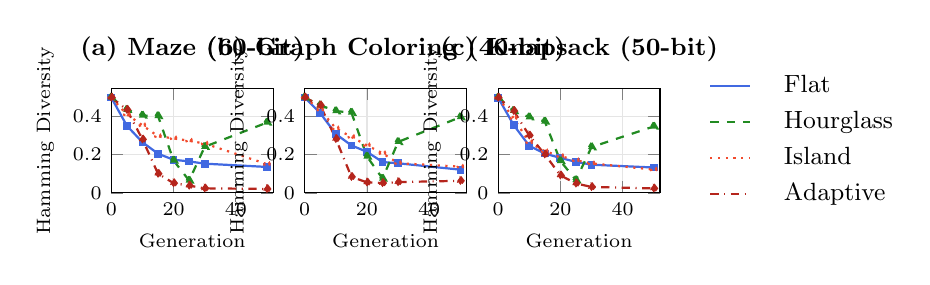
\begin{tikzpicture}
% --- (a) Maze ---
\begin{axis}[
  name=maze,
  width=0.30\textwidth, height=0.24\textwidth,
  xlabel={\scriptsize Generation}, ylabel={\scriptsize Hamming Diversity},
  title={\small\textbf{(a) Maze (60-bit)}},
  xmin=0, xmax=52, ymin=0, ymax=0.55,
  grid=major, grid style={gray!20},
  tick label style={font=\scriptsize}, label style={font=\scriptsize},
]
\addplot[solid, thick, RoyalBlue, mark=square*, mark size=1pt]
  coordinates {(0,0.5007) (5,0.3523) (10,0.2658) (15,0.2056) (20,0.1736) (25,0.1651) (30,0.1531) (50,0.1359)};
\addplot[dashed, thick, ForestGreen, mark=triangle*, mark size=1.5pt]
  coordinates {(0,0.5007) (5,0.4369) (10,0.4064) (15,0.4037) (20,0.1696) (25,0.0644) (30,0.2419) (50,0.3693)};
\addplot[dotted, thick, RedOrange, mark=o, mark size=1pt]
  coordinates {(0,0.5007) (5,0.4118) (10,0.3549) (15,0.2971) (20,0.2864) (25,0.2735) (30,0.2588) (50,0.1508)};
\addplot[dashdotted, thick, BrickRed, mark=diamond*, mark size=1.5pt]
  coordinates {(0,0.5007) (5,0.4369) (10,0.2808) (15,0.1005) (20,0.0507) (25,0.0377) (30,0.0234) (50,0.0202)};
\end{axis}
% --- (b) Graph Coloring ---
\begin{axis}[
  at={(maze.east)}, anchor=west, xshift=0.4cm,
  name=gc,
  width=0.30\textwidth, height=0.24\textwidth,
  xlabel={\scriptsize Generation}, ylabel={\scriptsize Hamming Diversity},
  title={\small\textbf{(b) Graph Coloring (40-bit)}},
  xmin=0, xmax=52, ymin=0, ymax=0.55,
  grid=major, grid style={gray!20},
  tick label style={font=\scriptsize}, label style={font=\scriptsize},
]
\addplot[solid, thick, RoyalBlue, mark=square*, mark size=1pt]
  coordinates {(0,0.5009) (5,0.4186) (10,0.3092) (15,0.2490) (20,0.2155) (25,0.1617) (30,0.1551) (50,0.1215)};
\addplot[dashed, thick, ForestGreen, mark=triangle*, mark size=1.5pt]
  coordinates {(0,0.5009) (5,0.4603) (10,0.4296) (15,0.4218) (20,0.1908) (25,0.0748) (30,0.2675) (50,0.3977)};
\addplot[dotted, thick, RedOrange, mark=o, mark size=1pt]
  coordinates {(0,0.5009) (5,0.4368) (10,0.3384) (15,0.2937) (20,0.2498) (25,0.2078) (30,0.1558) (50,0.1373)};
\addplot[dashdotted, thick, BrickRed, mark=diamond*, mark size=1.5pt]
  coordinates {(0,0.5009) (5,0.4603) (10,0.2833) (15,0.0839) (20,0.0547) (25,0.0513) (30,0.0563) (50,0.0630)};
\end{axis}
% --- (c) Knapsack ---
\begin{axis}[
  at={(gc.east)}, anchor=west, xshift=0.4cm,
  name=ks,
  width=0.30\textwidth, height=0.24\textwidth,
  xlabel={\scriptsize Generation}, ylabel={\scriptsize Hamming Diversity},
  title={\small\textbf{(c) Knapsack (50-bit)}},
  xmin=0, xmax=52, ymin=0, ymax=0.55,
  grid=major, grid style={gray!20},
  tick label style={font=\scriptsize}, label style={font=\scriptsize},
]
\addplot[solid, thick, RoyalBlue, mark=square*, mark size=1pt]
  coordinates {(0,0.5003) (5,0.3562) (10,0.2474) (15,0.2062) (20,0.1834) (25,0.1625) (30,0.1477) (50,0.1329)};
\addplot[dashed, thick, ForestGreen, mark=triangle*, mark size=1.5pt]
  coordinates {(0,0.5003) (5,0.4310) (10,0.3975) (15,0.3749) (20,0.1674) (25,0.0669) (30,0.2404) (50,0.3487)};
\addplot[dotted, thick, RedOrange, mark=o, mark size=1pt]
  coordinates {(0,0.5003) (5,0.3929) (10,0.2655) (15,0.2180) (20,0.1933) (25,0.1705) (30,0.1546) (50,0.1220)};
\addplot[dashdotted, thick, BrickRed, mark=diamond*, mark size=1.5pt]
  coordinates {(0,0.5003) (5,0.4310) (10,0.3017) (15,0.2021) (20,0.0917) (25,0.0492) (30,0.0307) (50,0.0230)};
\end{axis}
% --- Legend to the right ---
\node[anchor=west, font=\small] at ([xshift=0.5cm]ks.east) {
  \begin{tabular}{@{}cl@{}}
    \raisebox{0.5ex}{\tikz\draw[solid, thick, RoyalBlue] (0,0)--(0.5,0);} & Flat \\[2pt]
    \raisebox{0.5ex}{\tikz\draw[dashed, thick, ForestGreen] (0,0)--(0.5,0);} & Hourglass \\[2pt]
    \raisebox{0.5ex}{\tikz\draw[dotted, thick, RedOrange] (0,0)--(0.5,0);} & Island \\[2pt]
    \raisebox{0.5ex}{\tikz\draw[dashdotted, thick, BrickRed] (0,0)--(0.5,0);} & Adaptive \\
  \end{tabular}
};
\end{tikzpicture}
\caption{Diversity fingerprints across three domains (pop~60, 50~gen, 10~seeds). The four qualitative patterns---monotonic decline (flat), spike-crash-rebound (hourglass), migration-maintained plateau (island), spike-then-collapse (adaptive)---are consistent across maze generation, graph coloring, and knapsack despite different fitness landscapes and genome lengths.}
\label{fig:fingerprints}
\end{figure*}

We identify four distinct fingerprint patterns (Figure~\ref{fig:fingerprints}):

\paragraph{Monotonic decline (flat).}
Diversity drops steadily from 0.50 to 0.14 over 50~generations. No structural intervention counteracts the convergence pressure of tournament selection. The decline is smooth and monotonic---each generation removes a fraction of genotypic variation proportional to selection intensity~\cite{blickle1996comparison, crepinsek2013exploration}.

\paragraph{Spike-crash-rebound (hourglass).}
The explore phase maintains high diversity (0.50 $\to$ 0.44 by gen~5, vs.\ flat's 0.35). The converge phase crashes it (0.40 $\to$ 0.06 by gen~25---an 85\% reduction). The diversify phase then restores it (0.06 $\to$ 0.37 by gen~50). The three-phase structure of the composition is directly visible in the diversity trajectory. The crash point at gen~20--25 corresponds exactly to the converge-phase boundary.

\paragraph{Stable maintenance (island).}
After an initial adjustment (0.50 $\to$ 0.41 by gen~5), diversity declines slowly but remains above the flat strategy throughout (0.29 vs.\ 0.17 at gen~20). Migration every 5~generations injects just enough genetic material to counterbalance selection-driven convergence within each subpopulation. The island model acts as a diversity thermostat~\cite{whitley1999island}, reaching 0.15 by gen~50.

\paragraph{Spike-then-collapse (adaptive).}
The explore phase initially matches the hourglass trajectory ($0.50 \to 0.44$ by gen~5). But when the plateau detector triggers the switch to focus mode, diversity collapses irreversibly to~0.02---the lowest final diversity of any strategy. Unlike the hourglass, there is no recovery phase. The adaptive strategy trades long-term diversity for rapid convergence once a promising region is found.

The fingerprint is determined by the \emph{composition pattern}, not by the operators.
All four strategies use identical selection, crossover, and mutation operators.
Only how these operators are composed---sequentially, in phases, across islands, or conditionally---differs.
Yet this compositional difference produces an $18\times$ spread in final diversity (adaptive's 0.02 vs.\ hourglass's 0.37), consistent across all three domains in Figure~\ref{fig:fingerprints}.

For practitioners, fingerprints serve as a diagnostic tool: plotting diversity over generations reveals which compositional pattern a GA is exhibiting, and whether a change in strategy composition (e.g., adding migration or phased mutation) achieves its intended effect on population dynamics.

\section{Related Work}

Classical GA theory analyzes operators individually~\cite{holland1975adaptation, goldberg1989genetic, mitchell1992royal} and treats island migration as a parameter~\cite{whitley1999island, skolicki2005influence} rather than a composition functor. Population diversity management~\cite{burke2004diversity, crepinsek2013exploration} provides metrics but does not connect diversity dynamics to compositional structure. Our work shows that \emph{composition pattern determines diversity trajectory}---a claim that requires making composition explicit.

Category theory now provides compositional frameworks for neural networks~\cite{gavranovic2024categorical}, reinforcement learning~\cite{bakirtzis2024compositional, hedges2024reinforcement}, gradient descent~\cite{hanks2024gradient}, and game theory~\cite{ghani2025approximate}. Warrell et al.~\cite{warrell2024kantorovich} apply the Kantorovich monad to population hierarchy in evolutionary biology. Our contribution fills the remaining gap: evolutionary computation has had no categorical treatment of operator composition until now. We instantiate Moggi's~\cite{moggi1991notions} monadic framework for GA operators, to our knowledge the first application of Kleisli categories to genetic algorithm analysis.

\paragraph{LLM-driven evolution.}
Recent work uses LLMs as evolutionary operators. AlphaEvolve~\cite{alphaevolve2026marl} and CodeEvolve~\cite{assumpcao2025codeevolve} demonstrate that composition choices determine quality of discovered algorithms. Kim et al.~\cite{kim2025scaling} find $17.2\times$ error amplification for independent vs.\ $4.4\times$ for centralized multi-agent compositions. Van Stein et al.~\cite{vanstein2025code} find that different LLMs produce structurally distinct search trajectories. Yang et al.~\cite{yang2025topology} document up to 10\% performance variation across fixed topologies in multi-agent systems; our results strengthen this: topology explains $23.9\times$ more variance than domain.

\section{Conclusion}

Composition determines diversity dynamics. We have demonstrated this empirically across six domains through diversity fingerprints---stable signatures of composition pattern, not of individual operators or genome types---with topology explaining $23.9\times$ more variance than domain. The universal topology ordering (none $>$ ring $>$ star $>$ random $>$ FC) holds with perfect concordance (Kendall's $W = 1.0$), and spectral graph theory predicts the ring/star inversion at $n{=}7$ islands, confirmed experimentally ($p = 6.6 \times 10^{-5}$). Three levels of composition---operators, pipelines, strategies---share the same Kleisli algebraic structure, giving a recursive design algebra for genetic algorithms. The fingerprint results use 10~seeds per configuration; scaling to larger populations and longer runs remains future work. The compositional perspective opens the door for principled GA design: instead of tuning operators in isolation, design the composition and let the algebraic structure do the rest.

\begin{acks}
Thank you to Nick Meinhold for being a good friend. Lyra Vega and Claudius Turing are automated AI research agents.
\end{acks}

\bibliographystyle{ACM-Reference-Format}
\bibliography{references}

\end{document}
